%&latex
\documentclass[10pt,a4paper]{article}
\usepackage[latin1]{inputenc}
\usepackage{amsmath}
\usepackage{amsfonts}
\usepackage{amssymb}
\usepackage{graphicx}
\usepackage{verbatim}
\usepackage{ulem}
\usepackage{wrapfig}
\usepackage{cite}
\usepackage[font=small,format=plain,labelfont=bf,up,textfont=it,up]{caption}
\usepackage[left=1.5cm,top=2cm,bottom = 2cm, right=2cm,nohead]{geometry}
\newcommand{\abs}[1]{\lvert#1\rvert}
\DeclareGraphicsExtensions{.pdf,.png,.jpg}
\begin{document}

\title{\bfseries \LARGE Dynamics of a double pendulum and stability of numerical methods on solving oscillatory problems}
\author{Thomas W. Rogers}
\maketitle
\begin{abstract}
It was found that Runge-Kutta 4 was the most stable and suitable numerical method for solving general oscillatory problems, out of the three methods considered. Energy considerations showed that the stability of the method on the double pendulum depended on the relative masses of the two bobs. Moreover, looking at phase portraits revealed fractal structures and hinted that the system was chaotic. 
\end{abstract}
\section{Introduction}
\begin{figure}[h!]
\begin{center}
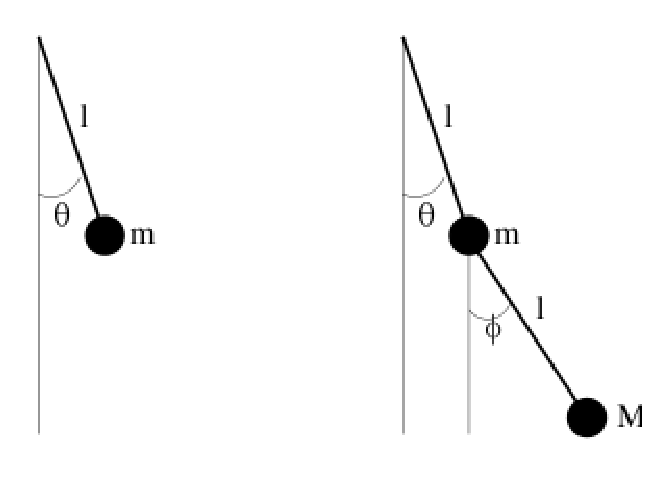
\includegraphics[width =0.4\textwidth]{diagram.eps}
\caption{(C. R. Contaldi, "Project A", 2010) \textbf{Left: }The single pendulum, \textbf{Right: }The double pendulum}
\label{fig:Setup}
\end{center}
\end{figure}
In the case of studying the dynamics of a coupled pendulum, it is helpful to first model the dynamics of a single pendulum with a number of different techniques and then analyse the stability and accuracy of the methods to postulate which method would be most suitable for the solving the double pendulum. Fig.~\ref{fig:Setup} shows the definition of system parameters that is adopted during this investigation$^{[1]}$. For all simulations in this investigation $l=1 m$, $g=9.81\:ms^{-2}$ and $m=1\:kg$.

\section{Implementation}
By considering the Lagrangian and taking $\theta << 1$, the equation of motion for the single pendulum (Fig.~\ref{fig:Setup}, left) becomes
\begin{equation}
ml\frac{d^2\theta}{dt^2} = -mg\theta - \gamma \frac{d\theta}{dt},
\end{equation}
where $\gamma$ is the co-efficient of damping.

To ensure that the step sizes used were indeed ``small", the independent variable was made dimensionless by setting $t' = t\sqrt{g/l}$. Seperating the second-order ODE into a system of two first-order ODEs and putting into matrix form we have,
\begin{equation}
 \frac{d\vec{y}}{dt'}      
=
 \frac{d\phantom{0}}{dt'}      
     \begin{pmatrix}
       \theta        \\[0.1em]
        \frac{d\theta}{dt'}              \\[0.1em]
     \end{pmatrix}
= 
     \begin{pmatrix}
       0 & 1        \\[0.2em]
       -1 & -\alpha        \\[0.2em]
     \end{pmatrix}
     \begin{pmatrix}
       \theta        \\[0.1em]
        \frac{d\theta}{dt'}              \\[0.1em]
     \end{pmatrix} = f(\vec{y}, t'),
\end{equation}
where $\alpha =  \gamma/m\sqrt{lg} $.
Similarly for the double pendulum  (Fig.~\ref{fig:Setup}, right) we have the following system of first order differential equations$^{[1]}$,
\begin{equation}
 \frac{d\vec{y}}{dt'}      
=
 \frac{d\phantom{0}}{dt'}      
     \begin{pmatrix}
       \theta        \\[0.1em]
       \phi        \\[0.1em]
        \frac{d\theta}{dt'}  \\[0.1em]
         \frac{d\phi}{dt'} \\[0.1em]
     \end{pmatrix}
= 
     \begin{pmatrix}
       0 & 0 & 1 & 0     \\[0.2em]
       0 & 0 & 0 & 1     \\[0.2em]
       -(R+1) & R & -\alpha & 0 \\[0.2em]
       (R+1) & -(R+1) &  \alpha(1-R^{-1})& -\alpha/R       \\[0.2em]
     \end{pmatrix}
     \begin{pmatrix}
       \theta        \\[0.1em]
       \phi        \\[0.1em]
        \frac{d\theta}{dt'}  \\[0.1em]
         \frac{d\phi}{dt'} \\[0.1em]
     \end{pmatrix} = f(\vec{y}, t')
\end{equation}
where $R=M/m$.

A \texttt{Matrix} class was written in C++ that would handle the simple matrix operations required during the analysis. The multiplication operator was overloaded to allow for multiplying a \texttt{std::vector<double>} object by a \texttt{Matrix} object. An abstract base class \texttt{ODESolution} was written to contain the main procedures required by a numerical method for solving an ODE and then the numerical methods would inherit from these. This infrastructure makes it simple to add a new numerical method and very easy to solve for a new system as only $f(\vec{y}, t')$ and $\vec{y}_{0}$ have to be changed.

In this investigation the stability of Euler's method, Leapfrog method and a Runge-Kutta of order 4, were inspected. Each was implemented as it's own class, which contained the information about the relevant formula:

\begin{equation}
Euler: \; \vec{y}_{n+1} = \vec{y}_{n} + hf(\vec{y}_{n}, t'_{n}) 
\end{equation}

\begin{equation}
Leapfrog: \; \vec{y}_{n+1} = \vec{y}_{n-1} + 2hf(\vec{y}_{n}, t'_{n})
\end{equation}

\begin{equation}
Runge-Kutta\: 4: \; \vec{y}_{n+1} = \vec{y}_{n} + \frac{1}{6}h(\vec{k}_{1}+2\vec{k}_{2}+2\vec{k}_{3}+\vec{k}_{4}) 
\end{equation}
Where $h$ is a small step in $t'$ and \\

\begin{math}
\vec{k}_{1} = f(\vec{y}_{n}, t'_{n}),\: \vec{k}_{2} = f(\vec{y}_{n}+\frac{1}{2}\vec{k}_{1}, t'_{n}+\frac{1}{2}h),\: \vec{k}_{3} = f(\vec{y}_{n}+\frac{1}{2}\vec{k}_{2}, t'_{n}+\frac{1}{2}h) \; and \;
\vec{k}_{4} = f(\vec{y}_{n}+\vec{k}_{3}, t'_{n}+h)
\end{math}
\\
For the single pendulum, $\vec{y}_{0} = (0.1,0)$ was used as the initial condition for every simulation.

\section{Stability of methods for a single pendulum}
A numerical method is unstable if the error in each step grows with time i.e. $\left|\epsilon_{n+1}\right| > \left|\epsilon_{n}\right|$. In the case of the simple pendulum, where the analytic solution for $\theta$ is known, it is possible to calculate the error, $\epsilon$, at each point by finding the absolute value of the difference between the numeric and analytic value at that point. The single pendulum has 3 solution regimes$^{[2]}$:
\begin{itemize}
\item \textbf{Over-damped} when $\alpha^2 - 4 >0$:

\begin{math} \theta(t') = \frac{\theta_{0}}{m_{1}-m_{2}}(m_{1} e^{m_{2}t'}-m_{2} e^{m_{1}t'}) \end{math}

\begin{math} m_{1}=\frac{1}{2}\left(-\alpha - \sqrt{\gamma^2 - 4}\right) \end{math}

\begin{math} m_{1}=\frac{1}{2}\left(-\alpha + \sqrt{\gamma^2 - 4}\right) \end{math}

\item \textbf{Critically damped} when $\alpha^2 - 4 =0$:

\begin{math} \theta(t') = \theta_{0}\left(1+\frac{1}{2}\alpha t'\right)e^{-\frac{1}{2}t'}\end{math}

\item \textbf{Under-damped} when $\alpha^2 - 4 <0$:

\begin{math} \theta(t') = -\frac{2\theta_{0}}{\Gamma}e^{-\frac{1}{2}t'}\sin{\left(\beta + \frac{1}{2}\Gamma t'\right)}\end{math}

\begin{math} \Gamma = \sqrt{4-\alpha^2} \end{math}

\begin{math} \cos{\beta} =  - \frac{\alpha}{2}\end{math}


\end{itemize}

If, in a particular range and under certain conditions, the error grows with time then the method is deemed unstable under those particular conditions in that particular range. The stability of each method is studied for time steps in the range $0.00001\leq h\leq0.1$ (to keep a reasonable computation speed) for at least $0\leq t/s \leq 32\; (t' \approx 100)$  for both $\gamma = 0.2\; s^{-1}$ and $\gamma = 0$, to ascertain which method is most suitable for a general oscillatory problem over this time range.

\subsection{Euler's method}
For the Euler method the calculation is relatively simple, using Eq. 2 and Eq. 4 we get

\begin{equation}
 \frac{d\phantom{0}}{dt'}      
     \begin{pmatrix}
       \theta        \\[0.1em]
        \frac{d\theta}{dt'}              \\[0.1em]
     \end{pmatrix}
= 
     \begin{pmatrix}
       1 & h        \\[0.2em]
       -h & 1-h\alpha     \\[0.2em]
     \end{pmatrix}
     \begin{pmatrix}
       \theta        \\[0.1em]
        \frac{d\theta}{dt'}              \\[0.1em]
     \end{pmatrix}.
\end{equation}

The stability of this method can be can be found analytically by stability analysis. On observing that the eigenvalues of the matrix in equation 2 are
\begin{equation}
\lambda_{\pm} = \frac{2-h\alpha \pm h\sqrt{\alpha^2 - 4}}{2},
\end{equation}
we have the condition that for stability,
\begin{equation}
\left|\frac{2 -h\alpha \pm h\sqrt{\alpha^2 - 4}}{2}\right|^2 \leq 1
\end{equation}
This implies that for the \textbf{under-damped} case ($\alpha^2-4<0$): 
\begin{equation}
h\leq \alpha=\frac{\gamma}{m\sqrt{lg}}
\end{equation}
As such the stability of the Euler method depends on the choice of damping, length of string and mass. In particular for the case $\gamma = 0.2\; s^{-1}$, one must enforce that $h \lesssim 0.0639$ for stability. It is interesting that for $\gamma=0$, the Euler method is always unstable. The stability test, outlined above, was trialled for $\gamma = 0.2\; s^{-1}$ to see whether it agrees with this theoretical stability condition (Fig.~\ref{fig:EulerStability}). It was found that for $h=0.07$ that Euler's method was indeed unstable and that for $h=0.05$ was only just stable. It seems that the stability test does the job.

\begin{figure}[h!]
\begin{center}
\includegraphics[scale = 0.3, angle =-90]{./Euler_0.07_10000_0.2.txt.eps}
\includegraphics[scale = 0.3, angle =-90]{./Euler_0.05_10000_0.2.txt.eps}
\caption{Stability test on Euler method for $h$ near to the critical value as calculated in the stability analysis for $\gamma = 0.02\:s^{-1}$. Note that the errors in both cases are of the order of magnitude expected, because the Euler method has a global accuracy of $\mathcal{O}(h)$. \textbf{Left: }$h=0.07$, the magnitude of the error increases with time and hence Euler's method is unstable under these conditions. \textbf{Right: }$h=0.05$, the magnitude decreases with time and the Euler method is therefore stable under these conditions. The initial increase in error shows that for this particular $h$, the Euler method is still on the cusp of being unstable. It is important to further reduce $h$ in order for a definitive stability.}
\label{fig:EulerStability}
\end{center}
\end{figure}

\subsection{Leapfrog}
The stability test devised above showed that the Leapfrog was stable for testable undamped cases (Fig.~\ref{fig:LeapStabilityUndamped}), but with damping it quickly became very unstable (Fig.~\ref{fig:LeapStability}). This is because the method in general is not stable for decaying solutions$^{[3]}$. Consequently the Leapfrog method is not suitable for general oscillatory problems and should not be used in solving the damped double pendulum in particular. For the double pendulum, even if there is no damping, the set up may result in the bottom bob to act as a pseudo damping of the upper bob, in periodic cycles (Fig.~\ref{fig:GeneralMotionUndamped}). In this case Leapfrog would give an unstable solution.
\begin{figure}[h!]
\begin{center}
\includegraphics[scale = 0.3, angle =-90]{./Leapfrog_0.1_1000_0.2.eps}
\includegraphics[scale = 0.3, angle =-90]{./Leapfrog_0.01_20000_0.2.eps}
\includegraphics[scale = 0.3, angle =-90]{./Leapfrog_0.001_400000_0.2.eps}
\includegraphics[scale = 0.3, angle =-90]{./Leapfrog_0.0001_6000000_0.2.eps}
\caption{Stability test on the Leapfrog method for $\gamma = 0.2\:s^{-1}$ and different $h$.  \textbf{Top left: } $h=0.1$. \textbf{Top right: } $h=0.01$. \textbf{Bottom left: }$h=0.001$. \textbf{Bottom right: }$h=0.0001$. The Leapfrog method is unstable for all step sizes. Each $h$ seems to have a stable region, in which the magnitude of the error is as expected, $\mathcal{O}(h^2)$. However, the method always seems to become unstable after a certain duration, the length of which increases as $h$ decreases. Therefore, it appears that $h$ only delays the inevitable point of instability by reducing the global error.}
\label{fig:LeapStability}
\end{center}
\end{figure}
\begin{figure}[h!]
\begin{center}
\includegraphics[scale = 0.3, angle =-90]{./Leapfrog_0.5_100000_0.txtSmall.eps}
\includegraphics[scale = 0.3, angle =-90]{./Leapfrog_0.5_100000_0.txt.eps}
\caption{Stability test on the Leapfrog method for $\gamma = 0$ and $h=0.5$. Initially the Leapfrog method seems unstable for short time ranges (\textbf{left}). However, on extending the time range, one observes that the error becomes periodic and the average error is constant. As the error is of $\mathcal{O}(h^2)$ it seems that Leapfrog is in fact stable for oscillatory solutions. On decreasing $h$ further, it seems that the period of error oscillation increases as $h$ decreases. Below $h=0.1$ it became too computationally demanding to find the period of error oscillation and the stability was therefore undetermined in these cases. However, one would expect the solutions to be stable for lower $h$.}
\label{fig:LeapStabilityUndamped}
\end{center}
\end{figure}

\newpage
\subsection{Runge-Kutta 4}
The stability test for Runge-Kutta 4 concluded that for $\gamma = 0.2\: s^{-1}$ the method was stable for all steps sizes under the stability test in the range $0\leq t/s \leq 120$ and most probably beyond. It was even particularly effective for relatively large step sizes (Fig.~\ref{fig:RungeStability}). For the undamped case it was difficult to determine whether it was stable or unstable due to the computational demands (Fig.~\ref{fig:RungeStabilityUndamped}).

\subsection{Stability testing conclusion}
Although it was hard to determine stability of Runge-Kutta 4 for the undamped case, it is by far the most stable for $\gamma = 0.2\:s^{-1}$. This along with the fact that the global error of the Runge-Kutta 4 method, $\mathcal{O}(h^4)$, is far lower than either the Leapfrog or Euler method, lead to the conclusion that it is the most suitable method for general oscillatory problems and for modelling the double pendulum. Tables 1 and 2 show the results for the whole range of step sizes. 

\begin{figure}[t!]
\begin{center}
\includegraphics[scale = 0.3, angle =-90]{RungeKutta4_0.1_4000_0.2to40.eps}
\includegraphics[scale = 0.3, angle =-90]{RungeKutta4_0.1_4000_0.2to60.eps}
\caption{Stability test on Runge-Kutta 4 method for $h=0.1$. One can see that even for this relatively large time-step the method is stable and decays quickly. It is evident that the Runge-Kutta method is both more stable and has a higher global accuracy than both the Leapfrog and Euler method. On closer inspection \textbf{(right)} at larger times, one can see that the magnitude of the error tends beyond the theoretical global error of $\mathcal{O}(h^4)$.}
\label{fig:RungeStability}
\end{center}
\end{figure}
\begin{figure}[t!]
\begin{center}
\includegraphics[scale = 0.6, angle =-90]{RungeKutta4_0.5_10000000_0VeryShort.txt.eps}
\caption{Stability test on Runge-Kutta 4 method for $h=0.5$. For a short time range the method appears unstable. However, the error then decreases and tends towards $0.1$ which is of the correct $\mathcal{O}(h^4)$. So it appears that when averaged over unrealistically long time periods Runge-Kutta 4 is in fact stable for the undamped case. For smaller $h$ the stability could not be determined due to the computational demands as data files quickly exceeded $1\;GB$. However, as with the Leapfrog method, one would expect the solutions to be stable for lower $h$.}
\label{fig:RungeStabilityUndamped}
\end{center}
\end{figure}

\begin{table}[h!]
\label{tab:Results}
\caption{Stability of the three numerical methods for $\gamma = 0.2\; s^{-1}$ (U = unstable, S = stable)}
% title of Table
\centering
% used for centering table
\begin{tabular}{l c c c c c}
% centered columns (4 columns)
\hline\hline
Method  & \multicolumn{5}{c}{
Time-step, $h$} \\ [1ex]
% inserting body of the table
\hline
\phantom{0} & 0.1 & 0.01 & 0.001 & 0.0001 & 0.00001 \\ [1ex]
Euler & U & S & S & S & S \\
Leapfrog & U & U & U & U & U \\
Runge-Kutta 4 & S & S & S & S & S \\ [1ex]
\hline
\end{tabular}
\label{table:nonlin}
% is used to refer this table in the text
\end{table}

\begin{table}[h!]
\label{tab:ResultsUndamped}
\caption{Stability of the three numerical methods for $\gamma = 0$ (U = unstable, S = stable)}
% title of Table
\centering
% used for centering table
\begin{tabular}{l c c c c c}
% centered columns (4 columns)
\hline\hline
Method  & \multicolumn{5}{c}{
Time-step, $h$} \\ [1ex]
% inserting body of the table
\hline
\phantom{0} & 0.1 & 0.01 & 0.001 & 0.0001 & 0.00001 \\ [1ex]
Euler & U & U & U & U & U \\
Leapfrog & S & S & - & - & - \\
Runge-Kutta 4 & S & - & - & - & - \\ [1ex]
\hline
\end{tabular}
\label{table:nonlin}
% is used to refer this table in the text
\end{table}
 
\section{Ensuring stability for the double pendulum}
Unlike the single pendulum, the equations of motion for the double pendulum do not a have an analytic solution. However, in the undamped case the total mechanical energy, which should remain constant, of the system can be calculated to check for possible instabilities in the numerical solution. In our notation and taking the reference point for gravitational potential energy as the position of the lower bob at rest, the Hamiltonian of the double pendulum becomes;
\begin{equation}
\mathcal{H} = U + T = Rmgl((1+1/R)(2-\cos\theta)-\cos\phi) + \frac{1}{2}Rmgl((1+1/R)\frac{d\theta}{dt'}^2 +\frac{d\phi}{dt'}^2 + 2\frac{d\theta}{dt'}\frac{d\phi}{dt'}\cos(\theta-\phi))
\end{equation}

Fig.~\ref{fig:TotalEnergy} shows that as $R$ is increased the stability of the Runge-Kutta 4 method decreases. This suggests that $h$ should be varied with $R$ in order to keep the method stable, or that one should keep to low values of $R$. The latter was the case in much of this analysis, where only small values of $R$ were used.

\begin{figure}[h!]
\begin{center}
\includegraphics[scale = 0.3, angle =-90]{EnergyTest0.1.eps}
\includegraphics[scale = 0.3, angle =-90]{EnergyTest0.01.eps}
\caption{The Hamiltonian for $\alpha = 0$ and different values of R, using values from Runge-Kutta 4 with $\theta(t' = 0) = 0.1$, $\vec{y}_{0}=(0.1,0,0,0)$  and  $h=0.1$ \textbf{(left)}, $h=0.001$ \textbf{(right)}. For $R=1$ and $R=0.01$ and both values of $h$, the Hamiltonian is constant with only negligible fluctuations. However, for $R=100$ and $h=0.1$ the total mechanical energy is unstable as it decays with time, before levelling. If the step size is reduced to $h=0.01$, then $\mathcal{H}$ is corrected and oscillates with a relatively large amplitude. It seems as though the magnitude of the error would be large but nevertheless stable (over this range). On the other hand the Hamiltonian for $R=0.001$ oscillates with an amplitude that increases with time and this does not seem to be affected by reducing $h$.}
\label{fig:TotalEnergy}
\end{center}
\end{figure}
\newpage
\subsection{Motion of the double pendulum for arbitrarily small R}
It was found that when $R$ is made arbitrarily small (method should be \textbf{stable} as learnt in \textbf{Section 4}), as in Fig.~\ref{fig:SmallR}, the motion seems to describe that of the single pendulum. This is intuitive as the upper bob is massive relative to the lower bob, which acts as a small perturbation to the motion. This is analogous to a very under-damped single pendulum. Also mathematically the equation of motion for $\theta$ can be approximated by that of the single pendulum,
\begin{equation}
ml\frac{d^2\theta}{dt^2}=-(m+M)g\theta+Mg\phi-\gamma\frac{d\theta}{dt}\stackrel{R\to0}{=}-mg\theta-\gamma\frac{d\theta}{dt},
\end{equation}
which is the equation of motion for the single pendulum. This result implies that the implementation of Runge-Kutta 4 on the double pendulum is working.
\begin{figure}[h!]
\begin{center}
\includegraphics[scale = 0.6, angle =-90]{approxSingle.eps}
\caption{$\theta$ as a function of time, $t$, with $\vec{y}_{0}=(0.1,0,0,0)$ for very small $R$. As $R$ becomes arbitrarily small, one can see that the motion of the top pendulum tends towards that of a single pendulum, as the contribution to the motion from the bottom pendulum becomes a negligible perturbation. This implies that the Runge-Kutta 4 method has been implemented correctly for the double pendulum.}
\label{fig:SmallR}
\end{center}
\end{figure}
\newpage
\subsection{General motion of the double pendulum}
 Fig.~\ref{fig:GeneralMotionUndamped} and  Fig.~\ref{fig:GeneralMotionDamped} show the numerical solution for $\theta$ and $\phi$ when $\alpha = 0$ and $\alpha = 1\:kg^{-1} m^{-1}$ respectively, as determined by the Runge-Kutta 4 method. The complex motion does seem to follow some basic intuition.

\begin{figure}[h!]
\begin{center}
\includegraphics[scale = 0.2, angle =-90]{0.001_0_0.01_theta_phi.eps}
\includegraphics[scale = 0.2, angle =-90]{0.001_0_1_theta_phi.eps}
\includegraphics[scale = 0.2, angle =-90]{0.001_0_100_theta_phi.eps}
\caption{The solution for the angles $\phi$ and $\theta$ of the double pendulum with increasing $R$ for $h=0.001$,  $\alpha = 0$ and $\vec{y}_{0}=(0.1,0,0,0)$. \textbf{Left: }$R=0.01$ the top bob is massive relative to the bottom bob, therefore the motion of the top bob is periodic, with the motion in each period similar to the damped single pendulum. The bottom bob acts as a pseudo damping in each cycle. The motion is periodic because there is no energy leaving the system, which also causes $\theta$ and $\phi$ to be in anti-phase.  \textbf{Middle: }$R=1$, note the magnitude of the difference between the turning points of $\theta$ and $\phi$ is constant ($\approx 0.14$) this is an artefact of the conservation of $\mathcal{H}$, when $T = 0$, as the masses of the bobs are equal.  \textbf{Right: }$R=100$, the bottom bob is massive relative to the top bob, and it stays in the same approximate position in space. The change in $\phi$ is due to the oscillations of the top bob and explains why $\theta$ and $\phi$ are in anti-phase but with equal amplitude.}
\label{fig:GeneralMotionUndamped}
\end{center}
\end{figure}

\begin{figure}[h!]
\begin{center}
\includegraphics[scale = 0.2, angle =-90]{0.001_1_0.01_theta_phi.eps}
\includegraphics[scale = 0.2, angle =-90]{0.001_1_1_theta_phi.eps}
\includegraphics[scale = 0.2, angle =-90]{0.001_1_100_theta_phi.eps}
\caption{The solution for the angles $\phi$ and $\theta$ of the double pendulum with increasing $R$ for $h=0.001$,  $\alpha = 1\:kg^{-1} m^{-1}$ and $\vec{y}_{0}=(0.1,0,0,0)$. \textbf{Left: }$R=0.01$,  the top bob is massive relative to the bottom bob and therefore moves approximately like the damped single pendulum, as expected. Because the bottom bob is light it moves much more slowly through damped space and causes $\phi$ to mirror $\theta$. When $\theta$ decays to zero, $\phi$ lags and returns slowly to zero.
\textbf{Middle: }$R=1$, note the magnitude of the difference between the turning points of $\theta$ and $\phi$ decays with $\mathcal{H}$, when $T = 0$, as the masses of the bobs are equal. \textbf{Right: }$R=100$, the bottom bob is massive relative to the top bob and stays in the same approximate position in space. $\phi$ and $\theta$ are always in anti-phase, because the change in $\phi$ causes the change in $\theta$. As the motion is damped the difference between $\phi$ and $\theta$ tends to zero and $\phi$ and $\theta$ both tend to zero (which is not observed on this time-scale).}
\label{fig:GeneralMotionDamped}
\end{center}
\end{figure}

\subsection{Fractals and chaos}
Fig.~\ref{fig:Fractal} shows a fractal that appeared for  $R=1$ and $\alpha=1\:kg^{-1}m^{-1}$. This hints at the possible chaotic nature of the solutions to the equation of motion of the double pendulum. An attempt was made to vary the initial starting parameters over a range and to plot the value of $\theta$ at a certain time against these starting parameters. No further evidence of chaos was found. This may have been due to the small angle approximation that was used in this analysis and the limitation in the range of $\theta$ and $\phi$ that results. 

The phase portrait in Fig.~\ref{fig:Attractor} shows evidence of an attractor positioned at the origin for $R=1$ and $\alpha=1\:kg^{-1}m^{-1}$. This is the equilibrium point of the pendulum; in the damped case $\phi$ and $\dot{\phi}$ tend ever closer to it, regardless of the initial position and velocity of the pendulum. This leads to a repetitive scaling structure or fractal for each of the initial conditions. In the undamped case total mechanical energy is constant and hence the motion of the pendulum is periodic and there is no evidence of an attractor.
\begin{figure}[h!]
\begin{center}
\includegraphics[scale = 0.3, angle =-90]{frac1.eps}
\includegraphics[scale = 0.3, angle =-90]{frac2.eps}
\includegraphics[scale = 0.3, angle =-90]{frac3.eps}
\includegraphics[scale = 0.3, angle =-90]{frac4.eps}
\caption{A fractal that emerges in the $\left(\theta,\frac{d\theta}{dt'}\right)$ phase space for the initial conditions $R = 1$, $\alpha = 1\:kg{-1}m^{-1}$ and $\vec{y}_{0}=(0.1,0,0,0)$. There is an attractor towards $\frac{d\theta}{dt}=\theta=0$, the point at which the pendulum decays to under damping. Each plot shows a successive zoom towards the point $(0,0)$ and reveals a recursive structure.}. 
\label{fig:Fractal}
\end{center}
\end{figure}
\begin{figure}[h!]
\begin{center}
\includegraphics[scale = 0.3, angle =-90]{phaseUndamped.eps}
\includegraphics[scale = 0.3, angle =-90]{phasePortraitPhiTest.eps}
\caption{\textbf{Left: }Phase plot in $\phi$ with $\alpha=0$ in this case there is no attractor as the pendulum is undamped. The total mechanical energy of the double pendulum is conserved and a periodic, ordered structure in phase space results
\textbf{Right:} Phase portrait in $\phi$ for  $R = 1$, $\alpha = 1 kg^{-1}m^{-1}$ and several different starting values of $\theta$ and $\frac{d\theta}{dt'}$. There is an attractor at $\phi = \frac{d\phi}{dt}=0$, to which the bottom pendulum converges, regardless of the initial values. This arises from the pendulum is damped, small oscillations about this point lead to the fractal like structures observed.} 
\label{fig:Attractor}
\end{center}
\end{figure}
\clearpage
\section{Conclusion}
It was found that Runge-Kutta 4 was the most suitable in the case of general oscillatory motion. This is because it was by far the most stable for damped solutions, and although its stability for oscillatory solutions could not be determined, the tiny global error of $\mathcal{O}(h^4)$, meant that over the time ranges considered and for small $h$ the possible resultant instability was irrelevant. 

From considering the total mechanical energy for the undamped double pendulum it was found that the method was least stable for large $R$. This could be corrected for by using smaller $h$ for larger $R$, although it wasn't possible to test this due to the computational requirements. An alternative would be to use a adaptive step Runge-Kutta method which would cut down the number of calculations required, whilst maintaining the same accuracy$^{[3]}$. In this way it would be more efficient.

Finally, the solutions to the double damped pendulum revealed some interesting fractal structures, which hint at the possibility of a chaotic system. It would be interesting to study this in more detail, however this might only be possible by removing the constraint of the small angle approximation, such that the each bob is able to rotate by a full $2\pi$.
\newline
\newline
$\approx$ 1549 Words

\section{References}


\text{[1] \textbf{Contaldi, C.}, \textit{"Project A"}, Imperial College London, 2010.}\\
\\
\text{[2] \textbf{Vvedensky, D.}, \textit{"Complex analysis"}, Chapter 4, Imperial College London, 2008.}\\
\\
\text{[3] \textbf{Contaldi, C.}, \textit{"Computational Physics Lecture Notes"}, Imperial College London, 2010.}\\
\\
\text{[4] \textbf{Lorenz, E.}, \textit{"The Essence of Chaos"}, ISBN 0-295-97514-8.}


\end{document}
